

\section{Preliminary Results}
\label{sec:preliminary}

As visualized in \reffig{fig:method}, two steps of this proposed methodology has already been carried out: A small-scale wasm application, and the basics of a browser-based visual programming language. These where both part of the preliminary work done in preparation of this thesis proposal. This chapter will elaborate upon these works.


\subsection{Wasm Application}
\label{sec:preliminary-wasm}

WebAssembly is a major component of this proposed thesis. However, the compilation target is still widely regarded as being "bleeding edge" \cite{jangda_not_2019}. This makes it all the more vital to gain some level of experience using the compile target before using it in more complicated scenario's. 

The Geomatics curriculum this thesis proposal is part of, offers a subject called "Research Assignment". This course offers students to gain experience in a geomatics-related topic of choice, and this made it the perfect context to try out WebAssembly for a geomatics web application.

The assignment given was to deliver a prototype for an online cityJSON validator. 
WebAssembly was to be used to perform a very fast JSON schema check over a user submitted json, among other things. 
This assignment was carried out successfully, and the delivered prototype (\reffig{fig:cjval-prototype}) played a role in the official CityJSON validator (\reffig{fig:cjval-official}), which uses WebAssembly. 

\begin{figure}[!tbp]
    \centering
    \begin{minipage}[b]{0.45\textwidth}
      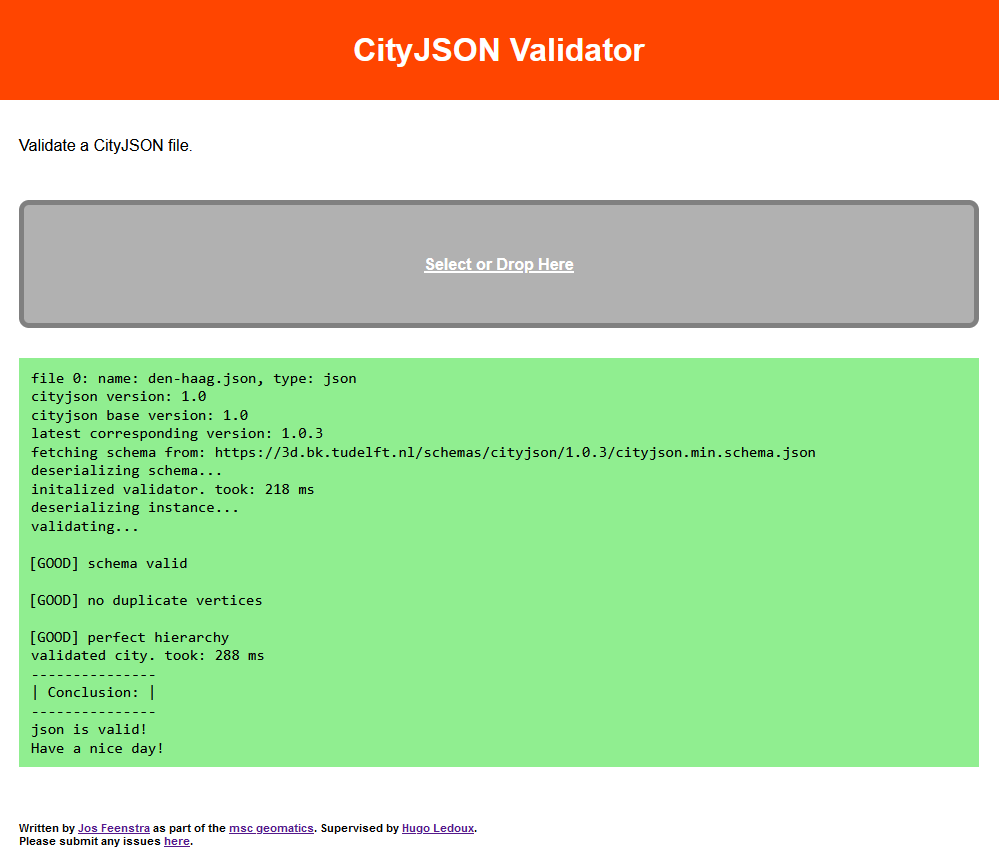
\includegraphics[width=\textwidth]{../images/cjval-prototype.PNG}
      \caption{The prototype}
      \label{fig:cjval-prototype}
    \end{minipage}
    \hfill
    \begin{minipage}[b]{0.45\textwidth}
      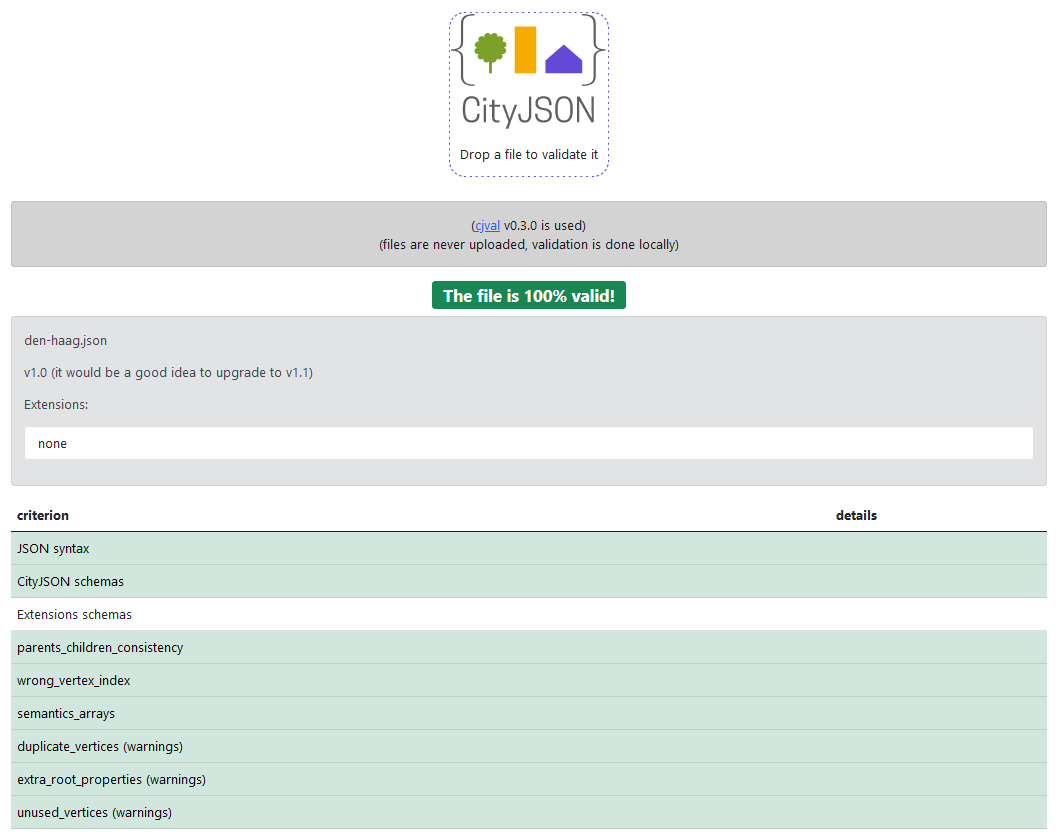
\includegraphics[width=\textwidth]{../images/cjval-official.PNG}
      \caption{The official validator}
      \label{fig:cjval-official}
    \end{minipage}
\end{figure}


Creating this application was very insightful. I would like to point out a few key insights, which will undoubtedly play an important role in the proposed thesis: 

\begin{itemize}

    \item The language this application was compiled from was Rust, not C++. Rust offers first-hand WebAssembly supports, as its default compiler supports WebAssembly. Surrounding tooling like \textit{wasm-pack} and community support \& tutorials made using WebAssembly within web applications very doable. 
    C++ will still be used in the proposed thesis for the sake of compiling existing libraries, but if the necessity arises to write custom WebAssembly components, Rust will be preferred, taking advantage of these aspects, and the fact that wasm can integrate multiple languages.

    \item It was very interesting to discover how WebAssembly supports a hybrid gui + cli setup. 
    The assignment was carried out by first developing a native Rust CLI-application which can be used as a standalone validator. 
    This code was then 'wrapped' as an api, and together with \textit{wasm-pack}, exposed and integrated within a website. 
    The advantage this offers is synergy between CLI and GUI. Any change made or feature added to the original application can easily be integrated within the web-exposed application. It also makes sure that a user can choose what interface they prefer. 

    % TODO diagram 

    \item The resulting application is extremely fast. It is one thing to theorize about performance gain, and another thing to experience it, and what it means for the usability of an application. The validation was often just as fast as the native binary application, and sometimes, for reasons not yet discovered, WebAssembly was even faster. When you start comparing this speed to other web-based json validators, this performance gain is even more apparent. A process which normally takes minutes now completes within a second. 

    % (TODO: maybe speed comparrison of https://jsonschemalint.com/#!/version/draft-07/markup/json
    % vs https://validator.cityjson.org/)

\end{itemize}


\subsection{VPL Prototype}
\label{sec:preliminary-vpl}

The question of what a FAIR geoprocessing interface should look like, together with partially implementing this interface, was the topic of a second preliminary study. 
As state before, this question's scope it wide, the question is difficult to proof, and can be considered slightly off-topic. We will therefore start from the presupposition that a web-based \ac{vpl} is a FAIR geoprocessing interface. This presupposition is informed by the following reasons: 

\begin{itemize}
  \item A \ac{vpl} can be seen as a compromise between a programming language and a full \ac{gui}. This has the advantage of serving both geodata experts, as well as the "data user" group depicted by \cite{brink_geospatial_2018}. The latter group might not be prepared to code, but would like to chain together geodata processing functions.
  \item \ac{vpl}'s have a clear advantage when dealing with data containing a visual component. Making in-between steps graphically debugable is very difficult to do with regular programming languages. Even programmers often use \ac{vpl}'s when programming shaders, for instance (SOURCE). 
  \item Geodata processing experts often depict geodata pipelines as a flowchart, graph, or a literal pipeline. 
\end{itemize}

Additionally, using a \ac{vpl} for geodata processing is not uncommon. examples of applications like these are FME, (SOURCE), QGIS's Model Builder (SOURCE), and Geoflow (SOURCE). Applications concerned with geometry manipulation in general also often choose \ac{vpl}'s, like Houdini(SOURCE), Blender's Geometry Nodes(SOURCE), and Rhino's Grasshopper(Source).


\subsubsection*{Design}

The way this \ac{vpl} was designed was influenced by the FAIR principles \cite{mark_d_wilkinson_fair_2016}, the analysis of exiting geo-vpl's mentioned above, as well as by and studies discussing the usability aspects of VPL's \cite{green_usability_1996, peters_geoflow_2019}. We present a MOSCOW analysis of the requirements of this environment: 

Must Have
\begin{itemize}
  \item Users must be able to configure their own graphs / flowchart. This involves \ac{ui} features like placing operations and drawing relationships between them. 
  \item This flowchart must be able to compute itself. This can be realized by using a \ac{dag}.
\end{itemize}

Should Have
\begin{itemize}
  \item The environment should support operations users have come to expect from applications in general, 
  like copy, paste, save, load, undo, redo, etc. 
  \item the environment should support GIS operations such as WFS, WMS, and CRS translations.
  \item The environment should support GIS input actions such as selecting coordinates on a map.  
  \item Created scripts should be able to run without the \ac{gui}. It would even be better to be able to compile the environment to plain JavaScript. 
  \item Created scripts should be sharable online by means of a link. This can be realized by either storing scripts on a server, or by saving to and loading scripts from a hash which can be included in a link. 
  \item Despite the goal of becoming a geoprocessing environment, we should enable the tool to additionally be used for acquiring, visualizing, and saving geodata.
 
\end{itemize}

Could Have
\begin{itemize}
  \item The environment could eventually be used completely offline again, like a normal, installable application, or a vscode plugin. Tools like 'electron' support this. 
  \item The environment could eventually support many input and output data formats, like cityJSON, .obj, and GLTF. 

\end{itemize}

Won't Have
\begin{itemize}
  \item The environment will not include a full IDE.
  \item The environment will not have login functionalities. The flowcharts will not be saved on a server.  
\end{itemize}



\subsubsection{Implementation}

This is how the development of this \ac{vpl} came to be. All Must haves's of the MOSCOW list have been completed, and a couple of should haves. The focus of the build was on the \ac{gui}, and as such, it supports only basic types. The environment is nicknamed 'GeoFront', as a concatenation of 'geoprocessing' and 'frontend'. 

\begin{figure}[!tbp]
  \centering
  \begin{minipage}[b]{1.0\textwidth}
    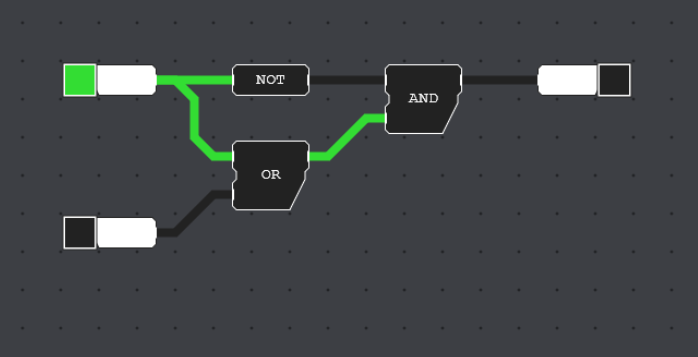
\includegraphics[width=\textwidth]{../images/geofront-1.PNG}
    \caption{The 'Geofront' environment. Source: Author}
    \label{fig:geofront-1}
  \end{minipage}
\end{figure}


\begin{figure}[!tbp]
  \centering
  \begin{minipage}[b]{1.0\textwidth}
    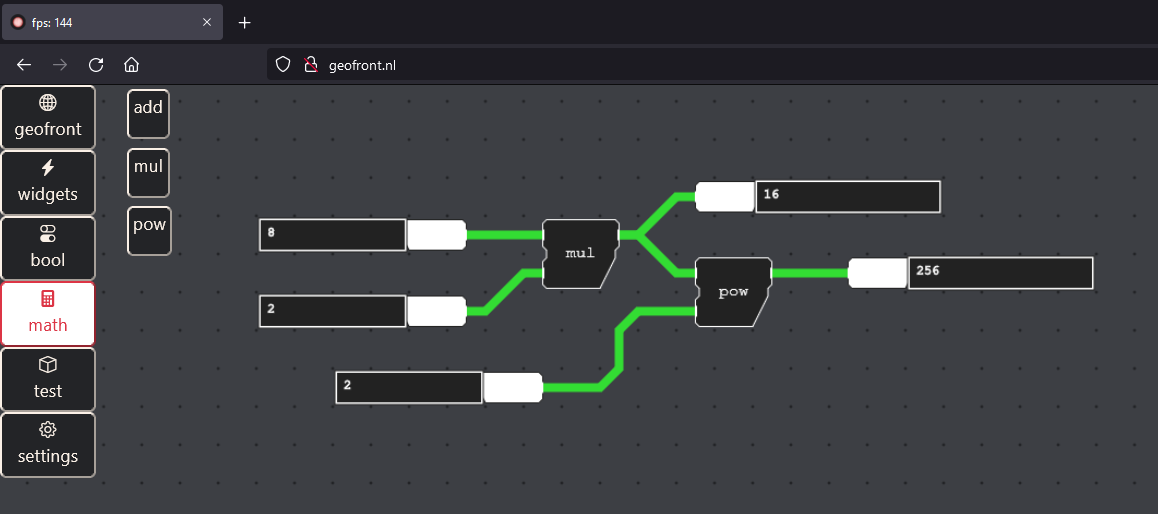
\includegraphics[width=\textwidth]{../images/geofront-2.PNG}
    \caption{GeoFront, showcasing basic mathematics. Source: Author}
    \label{fig:geofront-2}
  \end{minipage}
\end{figure}


The current application looks like \reffig{fig:geofront-1}. Input, output and operators can be placed on a canvas, and lines can be drawn in between these components. The graph then determines the order of execution by means of a \ac{dag}, and executes this any time an input has altered, or when the graph has been reconfigured. All graphics are provided by using the 2d Canvas API, native to modern web browsers.

Besides boolean values and operations, basic mathematical operations are also supported (see \reffig{fig:geofront-2}). Panels utilizing html are used to provide inputs and showcase outputs. 

\reffig{fig:geofront-3} shows how a graph can be saved as JavaScript. This script can be run completely independent of the geofront application, as long as the libraries used by the individual operation are included. The script can also itself be turned into an operation. This is meant for encapsulation, just like how regular programming languages support the creation and re-use of functions.

Lastly, \reffig{fig:geofront-4} shows that the first steps are made towards structs, objects, and other complex data types. 

\begin{figure}[!tbp]
  \centering
  \begin{minipage}[b]{1.0\textwidth}
    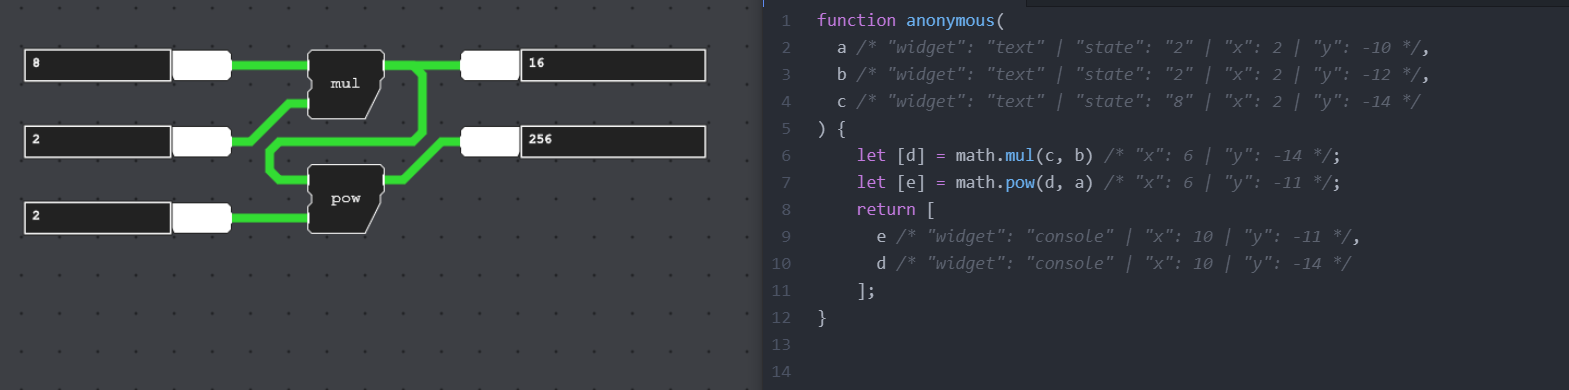
\includegraphics[width=\textwidth]{../images/geofront-3.PNG}
    \caption{GeoFront, showcasing javascript interoperability. Source: Author}
    \label{fig:geofront-3}
  \end{minipage}
\end{figure}

\begin{figure}[!tbp]
  \centering
  \begin{minipage}[b]{1.0\textwidth}
    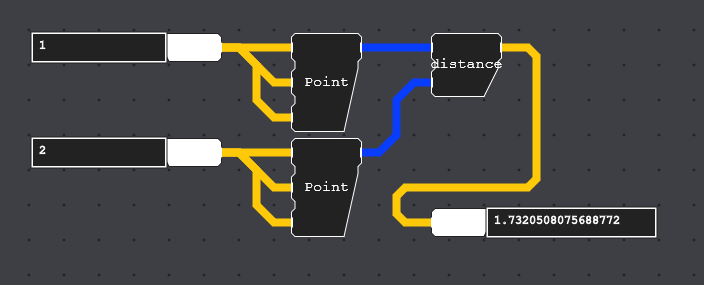
\includegraphics[width=\textwidth]{../images/geofront-4.PNG}
    \caption{GeoFront, showcasing support for basic structs. Types are color coded. Source: Author}
    \label{fig:geofront-4}
  \end{minipage}
\end{figure}